% !TEX encoding = UTF-8 Unicode
\documentclass[fontsize=11pt,paper=a4,titlepage,DIV=calc,draft=false]{scrreprt}
% 11pt: Normale Textkörpergröße
% a4paper: Größe des Druckmediums
% titlepage: Titel auf einer separaten Seite ohne Seitenzahl
% twoside: Zweiseitiges Layout
% openright: Kapitel beginnen immer auf der rechten Seite
% headsepline: Trennt Textkörper von Headings durch Strich (entspr.: /footsepline)
% headinclude,footinclude: Kopf- und Fußzeile zählen zum Textkörper
% DIV=calc: Für die gewählten Optionen wird ein optimales Seitenverhältnis errechnet
% draft=true: Für Bilder wird die Box freigehalten, erheblicher Geschwindigkeitsvorteil.
% abstract: Setzt den Titel 'Zusammenfassung' vor den abstract

% Blocktext in nahezu allen Situationen ermöglichen
\setlength\emergencystretch{.5\textwidth}

\usepackage{upgreek}
%\usepackage{subfigure}

%  %  %  %  Bindungskorrektour  %  %  %  %
% \KOMAoptions{BCOR=10mm}

%  %  %  %  Abkürzungen  %  %  %  %
% Das Einführen dieser Befehler verhindert Umbrüche bei mehrgliedrigen Abkürzungen
\usepackage{xspace}
\newcommand{\zB}{\mbox{z.\,B.}\xspace}
% Abkürzung für zum Beispiel


%  %  %  %  Einheiten  %  %  %  %
\usepackage[thinspace,thinqspace,squaren,textstyle]{SIunits}
% Komfoatables Paket zum Einbinden von Einheiten


%  %  %  %  Kodierung, Schrift und Sprache  %  %  %  %
\usepackage[utf8]{inputenc}
\usepackage{palatino}
\usepackage[ngerman]{babel}
% damit man Text aus dem PDF korrekt rauskopieren kann


%  %  %  %  Grafiken, Tabellen, Mathematikumgebungen  %  %  %  %
\usepackage{graphicx}
\usepackage{tabularx}
\usepackage{xcolor}
\definecolor{halfgray}{gray}{0.55}
\usepackage{amsmath,amsfonts,amssymb}
\usepackage{flafter,afterpage}
\usepackage[section]{placeins}
\usepackage{setspace} \onehalfspacing
\usepackage[margin=8mm,font=small,labelfont=bf,format=plain]{caption}
\usepackage[margin=8mm,font=small,labelfont=bf,format=plain]{subcaption}

\numberwithin{equation}{chapter}
\numberwithin{figure}{chapter}
\numberwithin{table}{chapter}

%  %  %  %  Kopf- und Fußzeilen  %  %  %  %

% \renewcommand\frontmatter{\pagenumbering{Roman}}
\usepackage{chngcntr}
\counterwithout{footnote}{chapter}

% Zeilenabstand zwischen zwei Fußnoten:
\footnotesep 9pt
% Einrücken der Fußnoten:
\deffootnote[1.5em]{1em}{1.5em}{\thefootnotemark\ \ }
%
%\usepackage{fancyhdr}				% Paket für leicht konfigurierbare Kopf- und Fußzeilen
%\fancypagestyle{plain}{				% Neue Gestaltung der Chapter- Page
%\fancyhf{} 							% Clear all header and footer fields
%\renewcommand{\headrulewidth}{0pt}		% Keine Trennlinie zwischen Kopf- / Fußzeile und Textkörper
%\renewcommand{\footrulewidth}{0pt}}
%
%\fancypagestyle{myfoot}{				% Neue Gestaltung der frontmatter pages
%\fancyhf{}							% Clear all header and footer fields
%\fancyhead[RO]{\thepage}				% Seitenzahl außen auf ungeraden Seiten
%\fancyhead[LE]{\thepage}				% Seitenzahl außen auf geraden Seiten
%\renewcommand{\headrulerwidth}{0pt}	% Keine Trennlinie zwischen Kopf- / Fußzeile und Textkörper
%\renewcommand{\footrulerwidth}{0pt}}
%
%\pagestyle{fancy}					% Pagestyle fancy aktiviert selbstkonfigurierten Style
%\fancyhf{} 							% Alle Kopf- und Fußzeilenfelder werden zunächst bereinig
%\renewcommand{\headrulewidth}{0pt}		% Keine Trennlienie zwischen Kopfzeile und Textkörper
%
%%\renewcommand{\chaptermark}[1]{\markboth{#1}{}}
%%\renewcommand{\sectionmark}[1]{\markright{#1}{}}
%
%\fancyhead[RO]{\leftmark ~~~~ \thepage}
%\fancyhead[LE]{\thepage ~~~~ \nouppercase \rightmark}


%  %  %  %  Überschriften  %  %  %  %


%  %  %  %  Verzeichnisse  %  %  %  %

% % % Literaturverzeichnis % % %
%\usepackage{natbib}

% % % Inhaltsverzeichnis % % %
% Die Chaptereinträge:
\usepackage{titletoc}

\titlecontents{chapter}
	[0pc]
	{
		\addvspace{0.5pc}
		%\filouter}
	}
	{\sffamily\Large\thecontentslabel\quad\sffamily\Large}{}
	{\titlerule*[0.75pc]{}\enskip\rmfamily\Large \contentspage}  % Wäre mit Seitenzahl 																					rechtsbündig
	[\addvspace{.5pc}]

% Die Sectioneinträge:
\titlecontents{section}
	[3.78em]
	{}
	{\rmfamily\contentslabel{2.3em}\rmfamily}
	{\hspace*{-2.3em}}
	{\titlerule*[0.75pc]{.}\enskip\contentspage}
	[\addvspace{.1em}]

% Die Subsectioneinträge:
\titlecontents{subsection}
	[6.2em]
	{}
	{\rmfamily\contentslabel{2.3em}\rmfamily}
	{\hspace*{-2.3em}}
	{\titlerule*[0.75pc]{.}\enskip\contentspage}
	[\addvspace{.1em}]

%\titlecontents{subsection}
	%[6.8em]
	%{}
	%{\rmfamily\normalsize\contentslabel{3em}\rmfamily\large}
	%{\hspace*{-2.3em}}
	%{\titlerule*[0.75pc]{.}\enskip\contentspage}
\begin{document}

%  %  %  %  Titelseite  %  %  %  %
\begin{titlepage}
	\vspace*{\fill}

	\rule{\textwidth}{0.25pt}

	\vspace*{1cm}

	\begin{singlespace}
		\begin{center} \Large \bfseries
			Rechnernetze/Kommunikationssysteme
		\end{center}
	\end{singlespace}

	\vspace{2em}

	\begin{singlespace}
		\begin{center} \bfseries
			Dokumentation zur Belegarbeit
		\end{center}
	\end{singlespace}

	\vspace*{6cm}

	\begin{center}
		vorgelegt von \\
		\vspace{2em}
		Leonard Hecker
	\end{center}

	\vspace*{1cm}

	\rule{\textwidth}{0.25pt}

	\vspace*{\fill}
\end{titlepage}

%  %  %  %  Inhaltsverzeichnis  %  %  %  %

\tableofcontents

%  %  %  %  Hauptteil  %  %  %  %

\chapter{Funktionsweise des Servers}

Nach der Erstellung eines UDP Sockets befindet sich der Server im sog. \textit{main loop} und wartet dort zu Beginn bis ein Paket empfangen wird in der \textit{receive} Methode des Sockets.
Wie im Protokoll festgelegt muss das erste Paket, einem Handshake entsprechen, weshalb alle Felder auf Konformität geprüft werden.
Neben einem Test der die Einhaltung der Grenzwerte von jedem Feld prüft muss auch die CRC32 Summe über alle Handshake-Felder, abgesehen vom CRC32 Feld selbst berechnet werden.
Ist die Prüfsumme die gleiche wie die im CRC32 Feld des Handshakes, so sendet der Server nun ein ACK an den Client
Ist eines der Felder jedoch invalide, oder aber die Prüfsumme ungleich, so wird kein ACK gesendet und an den Anfang des Programms gesprungen, wo der Server wieder auf einen validen Handshake wartet..
Zunächst erstellt der Server nun eine Datei mit dem im Handshake spezifizierten Namen.
Sollte die Datei bereits existieren, dann werden wie in der Aufgabenstellung gefordert alternative Namen getestet.
Wurde ein Name gefunden, so erstellt der Server damit eine neue, leere Datei, sendet dem Client ein ACK und springt in den \textit{data loop}.
Tritt ein Fehlerfall im \textit{data loop} ein, so wird die aktuelle Verbindung abgebrochen, die bereits erstellte Datei gelöscht und wieder zu dem Beginn des \textit{main loop} gesprungen.
Da zum Beginn des \textit{main loop} auf einen validen Handshake getestet wird und für invalide kein ACK gesendet wird, wird der Client nach 10 weiteren \textit{send}-Versuchen ohne ACKs durch einen Timeout abbrechen. \newline

Auch am Anfang des \textit{data loop} wartet der Server wieder in der \textit{receive} Methode des Sockets, bis ein Paket empfangen wird, oder ein Timeout eintritt.
Ein Timeout entspricht hierbei einem Fehlerfall.
Wurde ein Paket vom aktuellen Client, mit der selben IP, dem selben Port und der selben Sessionnummer, empfangen, so wird es wieder auf Konformität zum Protokoll getestet.
Stammt es von einem anderen Client, dann wird es ignoriert, jedoch nicht das Timeout zurückgesetzt.
Würde man dies tun, könnte man eine abgebrochene Übertragung beliebig lange mit Paketen anderer Clients in der \textit{data loop} Schleife festhalten.
Um die Validität des Paketes festzustellen, muss zunächst getestet werden ob die Sessionnummer die gleiche wie die im Handshake vereinbarte ist.
Ist sie nicht gleich, so ist dies ein Fehlerfall.
Wenn der Client ein ACK des Servers nicht erhalten hat, sendet dieser ein Datenpaket noch einmal, weshalb an dieser Stelle getestet werden muss, ob es sich bei der Paketnummer des Pakets um eine abgelaufene hält.
Falls dies der Fall ist ignoriert der Server den Paketinhalt, sendet das ACK für das vergangene Paket noch einmal und setzt am Anfang des \textit{data loop} fort.
Andernfalls kann man davon ausgehen, dass es sich um das nächste, neue Paket handelt, weshalb der Server nun das Timeout zurücksetzt.
Sollte das Paket mehr Daten enthalten, als noch geschrieben werden müssen, dann ist dies auch ein Fehlerfall.
Diese Menge der noch fehlenden Bytes lässt sich leicht aus der im Handshake angegebene Dateigröße und der Menge an bereits geschriebenen Bytes ermitteln.
Die Daten des Paketes, sofern welche vorhanden sind, werden nun in die bereits erstellte Datei geschrieben.
Ist die Menge der im Handshake vereinbarten Daten bereits geschrieben worden, so müssen in diesem Paket exakt 4 weitere Byte vorhanden sein.
Diese 4 Byte entsprechen dem CRC32 Feld im Protokoll und müssen mit der CRC32 Prüfsumme aller geschriebenen Daten übereinstimmen.
Eine ungleiche Prüfsumme gilt als Fehlerfall.
Ansonsten sendet der Server nun für das aktuelle Paket ein ACK und setzt falls noch Daten oder das CRC32 Feld fehlen im \textit{data loop} und andernfalls im \textit{main loop} fort. \newline

Um Netzwerke zu simulieren enthält der Server Funktion um Delay, Delay-Variation und Loss einzustellen.
Delay entspricht hierbei der mittleren Verzögerung in jeweils Sende- und Empfangsrichtung.
Mittels Delay-Variation kann man hierbei dem Delay eine scheinbare, um den Delay-Wert normalverteilte, Zufälligkeit beimischen.
Diese Verzögerung wird hierbei mittels einem Aufruf von \textit{sleep} auf dem Main-Thread erreicht und betrifft sowohl Sende- als auch Empfangsrichtung.
Ein Delay von \textit{100ms} führt somit zu einer RTT von \textit{200ms}.
Zuletzt ist es mittels Loss möglich Pakete mit einer bestimmten Wahrscheinlichkeit nicht zu empfangen, bzw. zu senden.
Wurde entschieden ob ein Paket als Loss gilt wird dieses einfach ignoriert und im Falle eines zu sendenden ACKs nichts unternommen, bzw. beim empfangen auf das nächste gewartet. \newline

\begin{figure}
	\centering
	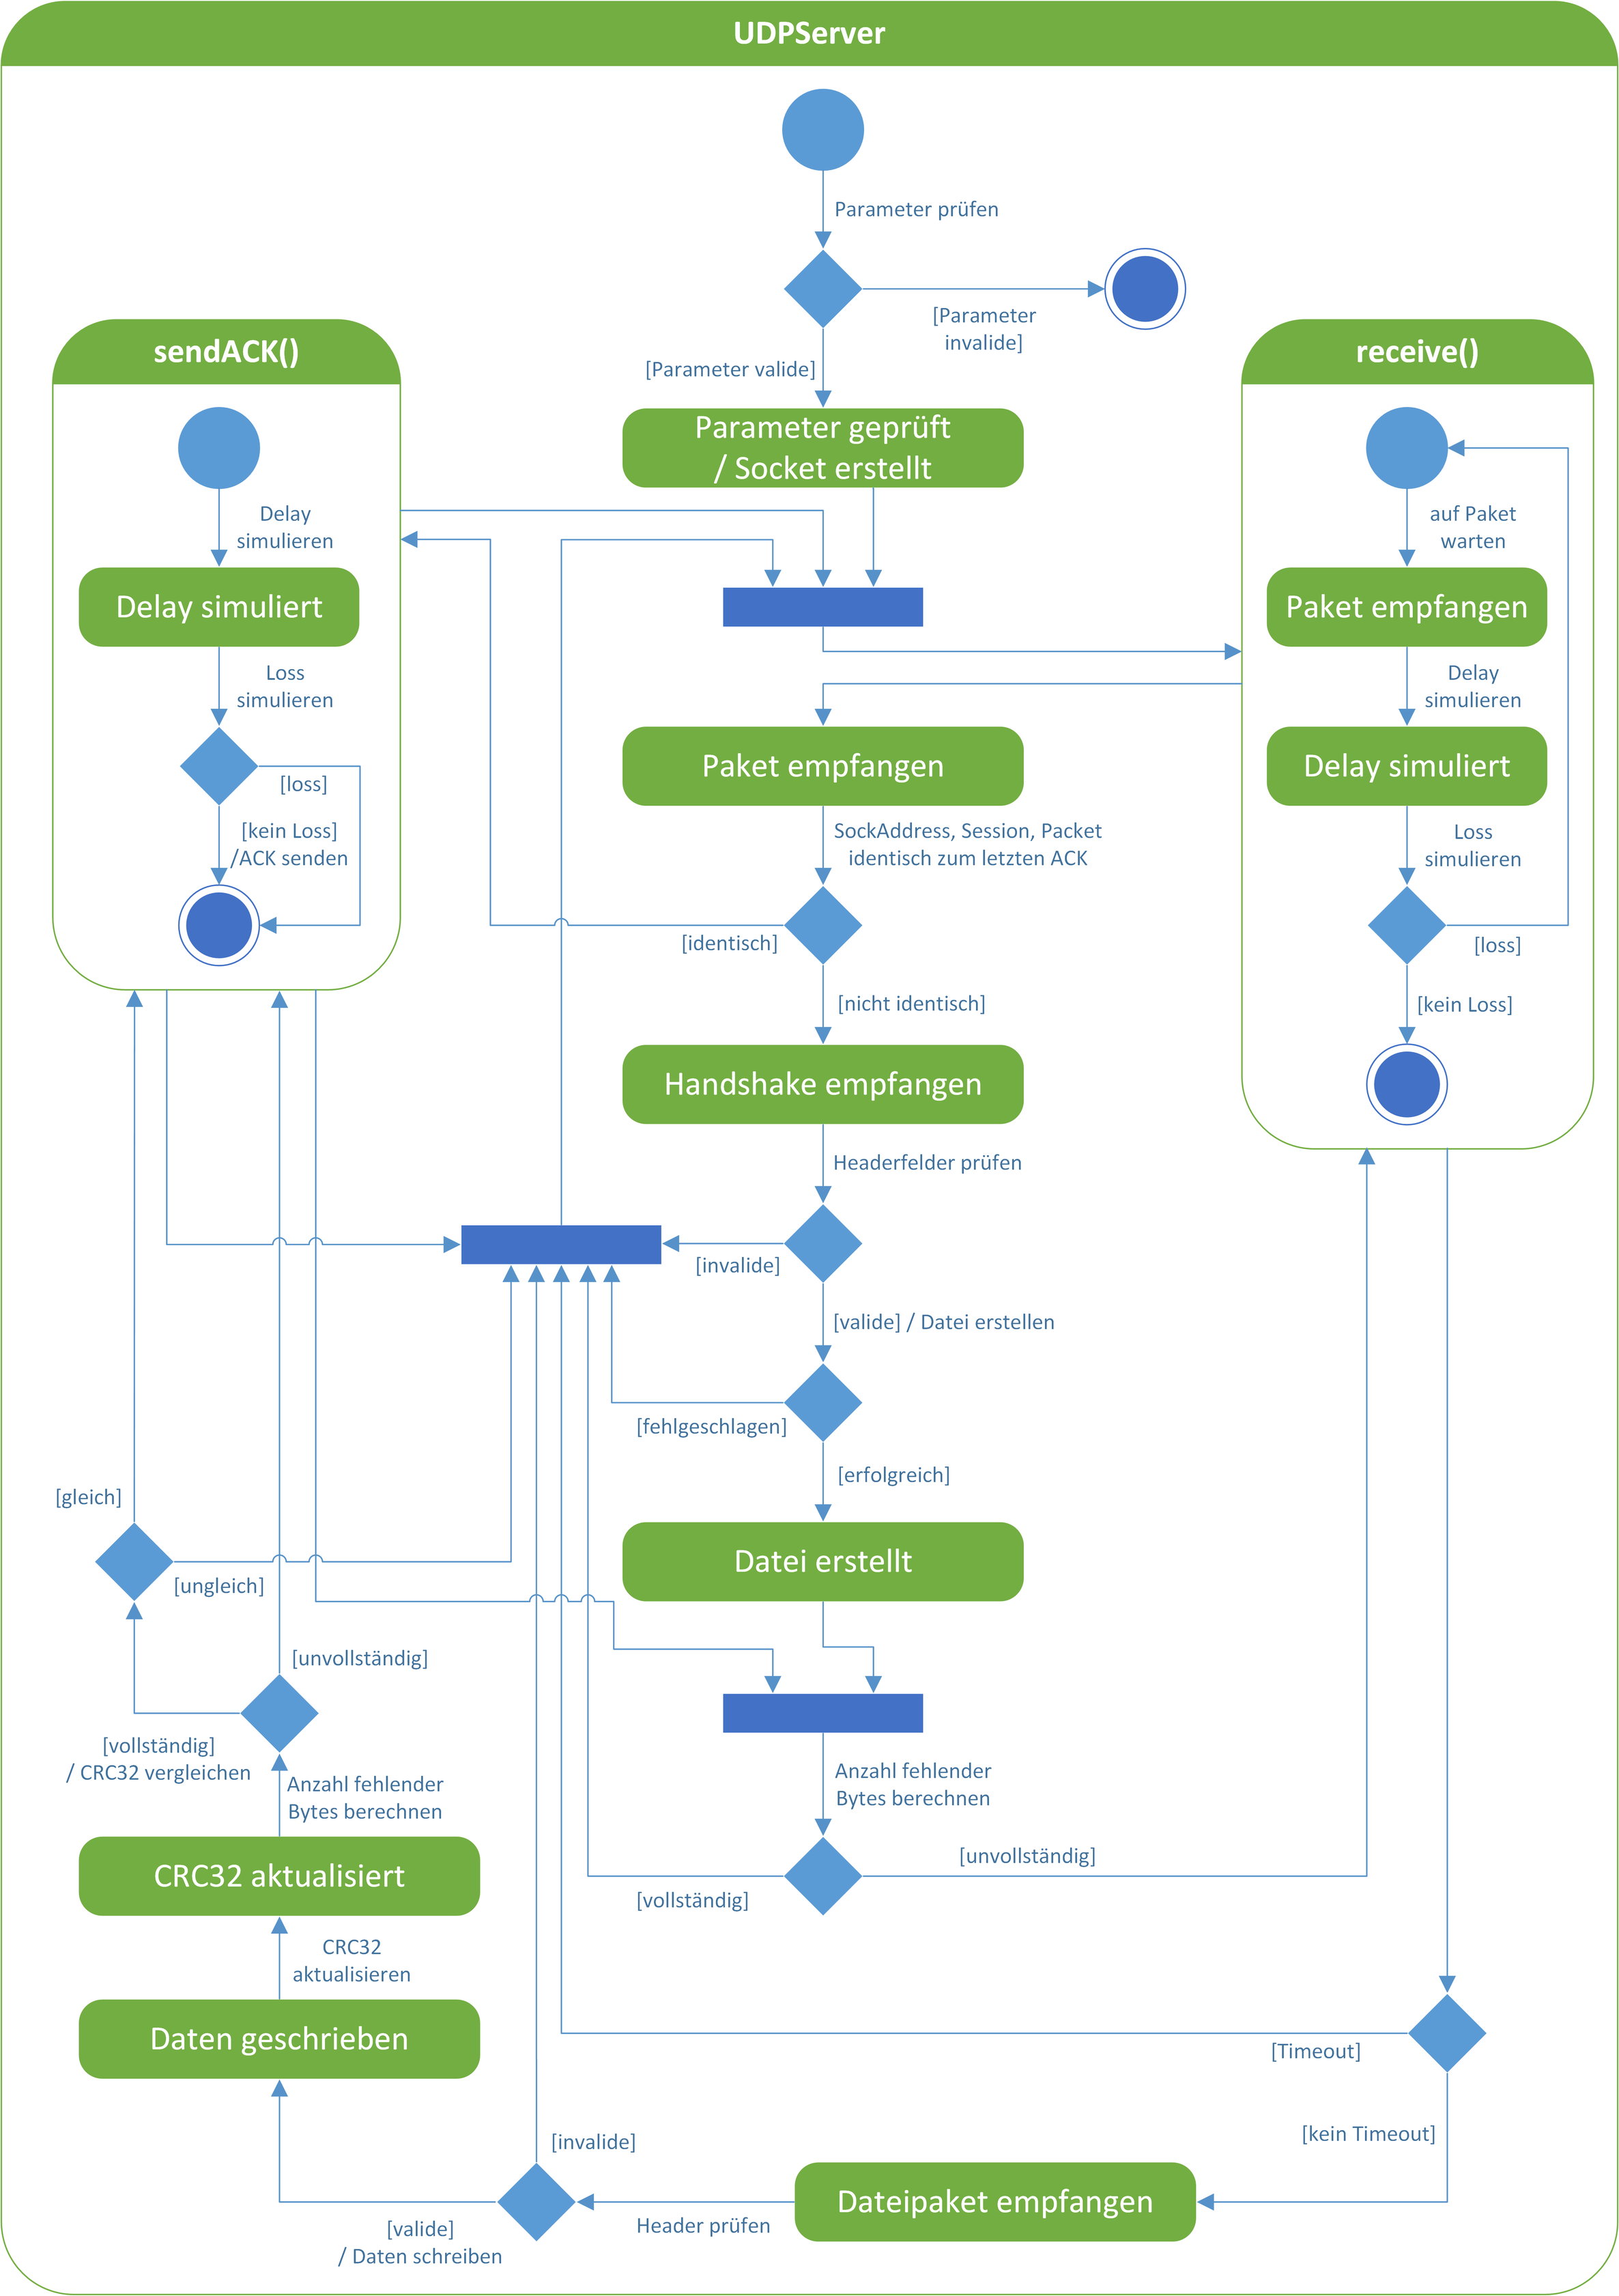
\includegraphics[width=\textwidth,height=\textheight,keepaspectratio]{assets/UDPServer.png}
	\caption{Zustandsdiagramm einer Dateiübertragung}
\end{figure}

\chapter{Funktionsweise des Clients}

Zunächst ist festzulegen, dass der Client bei einem Fehlerfall die Ausführung abbricht.
Sollte der angegebene Host und Port nicht auflösbar, oder die Datei unter dem angegebenen Namen nicht zu finden sein, dann ist dies ein Fehlerfall.
Da es für eine optimale Geschwindigkeit nötig ist die MTU bis zum Server zu kennen, wäre eine MTU Path Discovery nötig.
Da dies jedoch unter Java nahezu unmöglich ist wird die MTU hier angenähert.
Dies ist möglich indem man das minimum der MTU aller Network Interfaces findet.
Sollte dies jedoch fehl schlagen oder eine ungewöhnlich kleine MTU gefunden werden, so wird eine MTU von 576 Bytes angenommen.
Dies entspricht der im RFC 1122 als EMTU\_R festgelegten für Hosts kleinstmögliche MTU.
Da jedoch eine MTU die Größen von IPv4/v6-Headern usw. nicht einbezieht, müssen wir noch z.B. 48 Byte abziehen um die maximale Nutzdatengröße zu erhalten, was der Größe eines UDP Headers in einem IPv6 Header entspricht.
Zunächst wird ein Handshake-Paket gemäß dem vorgegebenen Protokoll erstellt.
Die Felder für die Länge des Dateinamens und der Dateiname selbst werden selbstverständlich mit dem Basename der bereits zu Beginn gefundenen Datei ausgefüllt.
Das Feld für den Dateinamen hat hierbei eine dynamische Größe und passt sich der Länge des Dateinamens an.
Das für die CRC32 Prüfsumme wird hingegen gemäß Protkoll mit der Prüfsumme über alle Handshake-Felder außer dem des CRC32-Feld's selbst ausgefüllt.
Ist das Handshake-Paket fertig so wird dieses an den Server geschickt und in den sog. \textit{data loop} gesprungen. \newline

Die \textit{send} Methode des Clients handhabt hierbei das Versenden von Daten.
In dieser Methode ist abstrahierten dabei das geforderte Verhalten, dass ein Paket bis zu 10 mal gesendet werden soll, falls kein ACK eintrifft.
Dies bedeuted, dass die \textit{send} Methode somit auch das empfangen von ACKs und die Berechnung von geeigneten Timeouts handhabt.
Das Timeout wird mittels einem Algorithmus berechnet, der dem des Retransmission Timer aus dem TCP Protokoll ähnlich ist.
Hier wird jedoch mit einer feineren Granulität von Millisekunden statt ganzen Sekunden gearbeitet.
Der minimale Timeoutwert liegt des Weiteren bei nur \textit{10ms} und der maximale nur bei \textit{3000ms}.
Dies ergibt sich daraus, dass dieses Projekt nur zu Demonstrationszwecken verwendet wird.
Tritt 10 mal hintereinander ein Timeout ein, so ist dies ein Fehlerfall.
Enthält das ACK des Servers eine invalide Sessionnummer, so ist das ein Fehlerfall.
Falsche Paketnummern werden hingegen als ein Timeout bewertet. \newline

Sollte der Client schneller senden, als der Server die Pakete aktuell empfängt, so würden sich diese aufstauen.
Da der Server für jedes empfangene Paket ein ACK sendet, so wird der Client nun für jedes aufgestaute Paket ein ACK erhalten.
Da der Client für jedes invalide Paket nun ein ACK senden würde, würde dieser wiederum genausoviele Pakete senden.
Man könnte so durch einen schnell sendenden Client also eine immer größere Anzahl an aufgestauten Paketen provozieren. \newline

Im \textit{data loop} wird nun zunächst der Header eines Datenpaketes gemäß dem Protokoll erstellt.
Dem Datenpaket wird nun die größtmögliche Menge an Daten, welche sequentiell aus der Datei ausgelesen wurden, angehangen.
Dies geschieht unter Beachtung der bereits ermittelten maximalen Payloadgröße und der Bedingung des Protokolls, dass die CRC32 Prüfsumme am Ende der Datei nicht auf mehrere Pakete aufgeteilt werden darf.
Die jeweilige Menge an Daten werden nun auf eine CRC32 Prüfsumme aufgerechnet.
Wurde die gesamte Datei in Datenpakete aufgeteilt wird nun die berechnete CRC32 Prüfsumme an das Ende des Paketes angehangen --- es ist hierbei auch möglich dass das finale Paket nur mit CRC32 und ohne Daten gesendet wird.

\begin{figure}
	\centering
	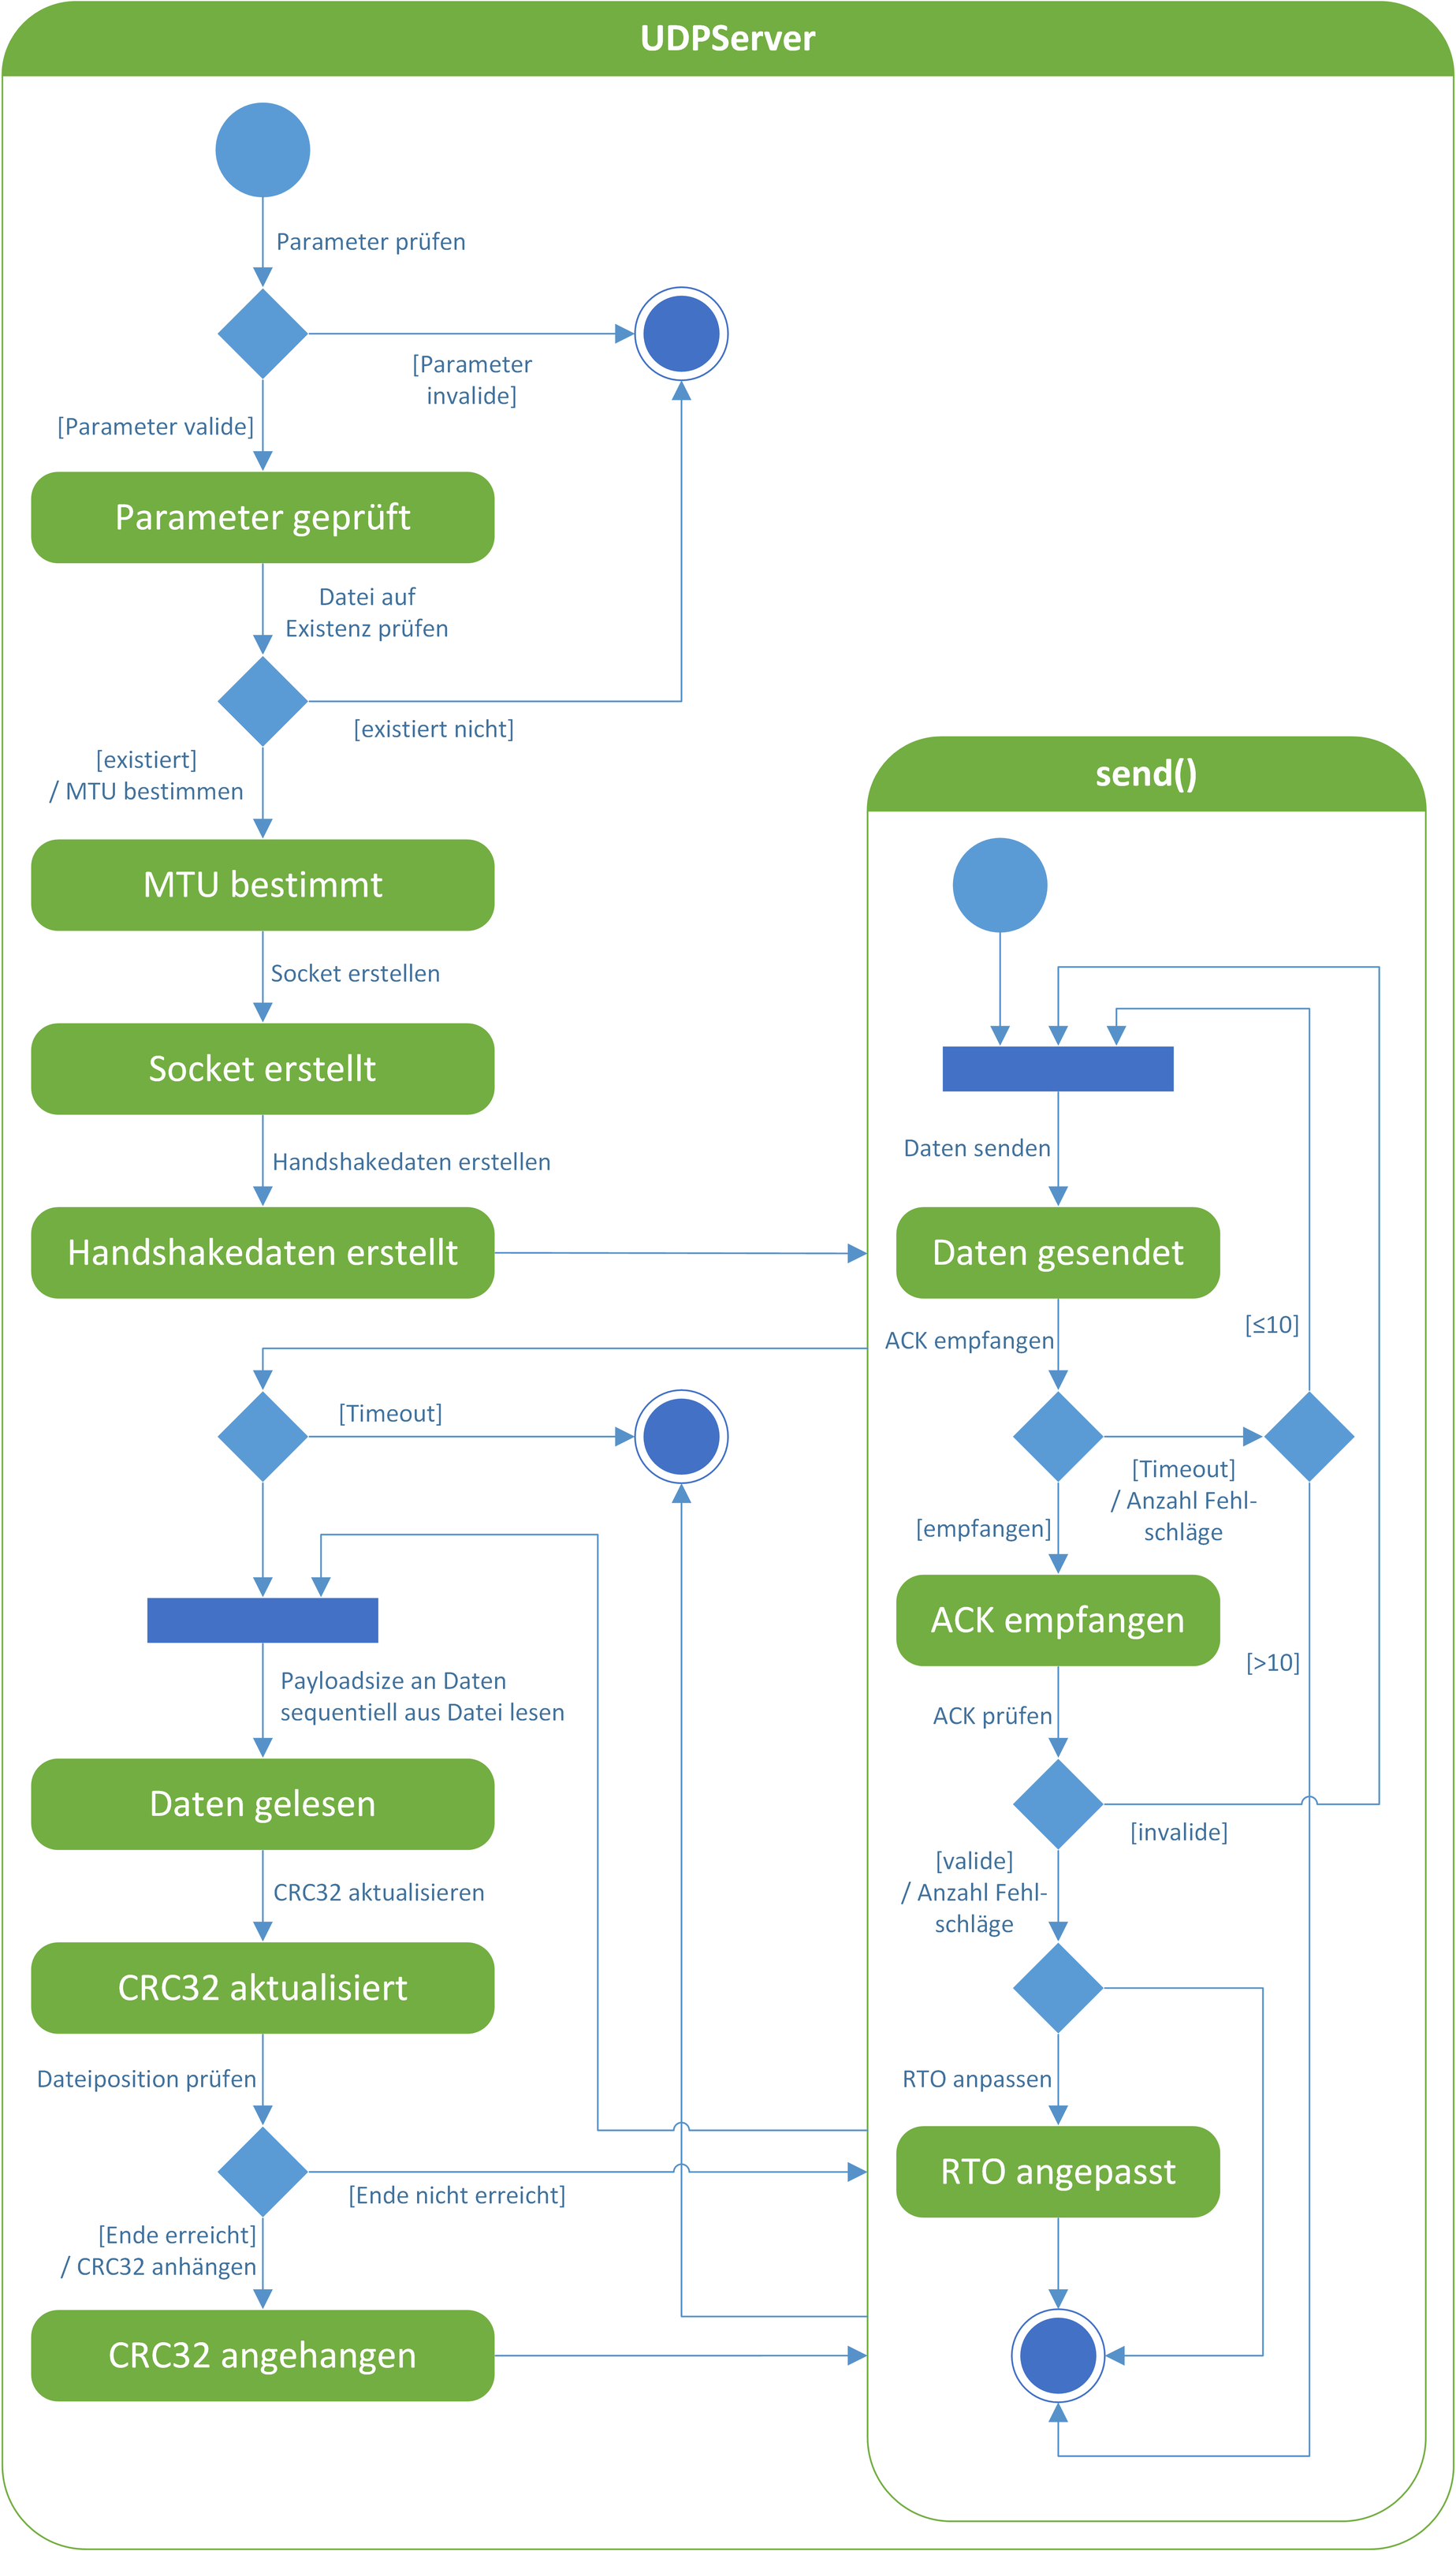
\includegraphics[width=\textwidth,height=\textheight,keepaspectratio]{assets/UDPClient.png}
	\caption{Zustandsdiagramm einer Dateiübertragung}
\end{figure}

\end{document}
